% This LaTeX was auto-generated from MATLAB code.
% To make changes, update the MATLAB code and export to LaTeX again.

\documentclass{article}

\usepackage[utf8]{inputenc}
\usepackage[T1]{fontenc}
\usepackage{lmodern}
\usepackage{graphicx}
\usepackage{color}
\usepackage{hyperref}
\usepackage{amsmath}
\usepackage{amsfonts}
\usepackage{epstopdf}
\usepackage[table]{xcolor}
\usepackage{matlab}
\usepackage[paperheight=795pt,paperwidth=614pt,top=72pt,bottom=72pt,right=72pt,left=72pt,heightrounded]{geometry}

\sloppy
\epstopdfsetup{outdir=./}
\graphicspath{ {./report_media/} }

\matlabhastoc

\begin{document}

\label{TMP_8ffc}
\vspace{1em}

\label{TMP_741c}
\matlabtitle{Pendulum cart control}

\begin{par}
\begin{flushleft}
The system consists of a cart of mass $M$ carrying a pendulum of mass $m$ through a mass-less rod with a length $l$ . The cart displacement is driven by a horizontal force u.  
\end{flushleft}
\end{par}

\begin{par}
\begin{center}
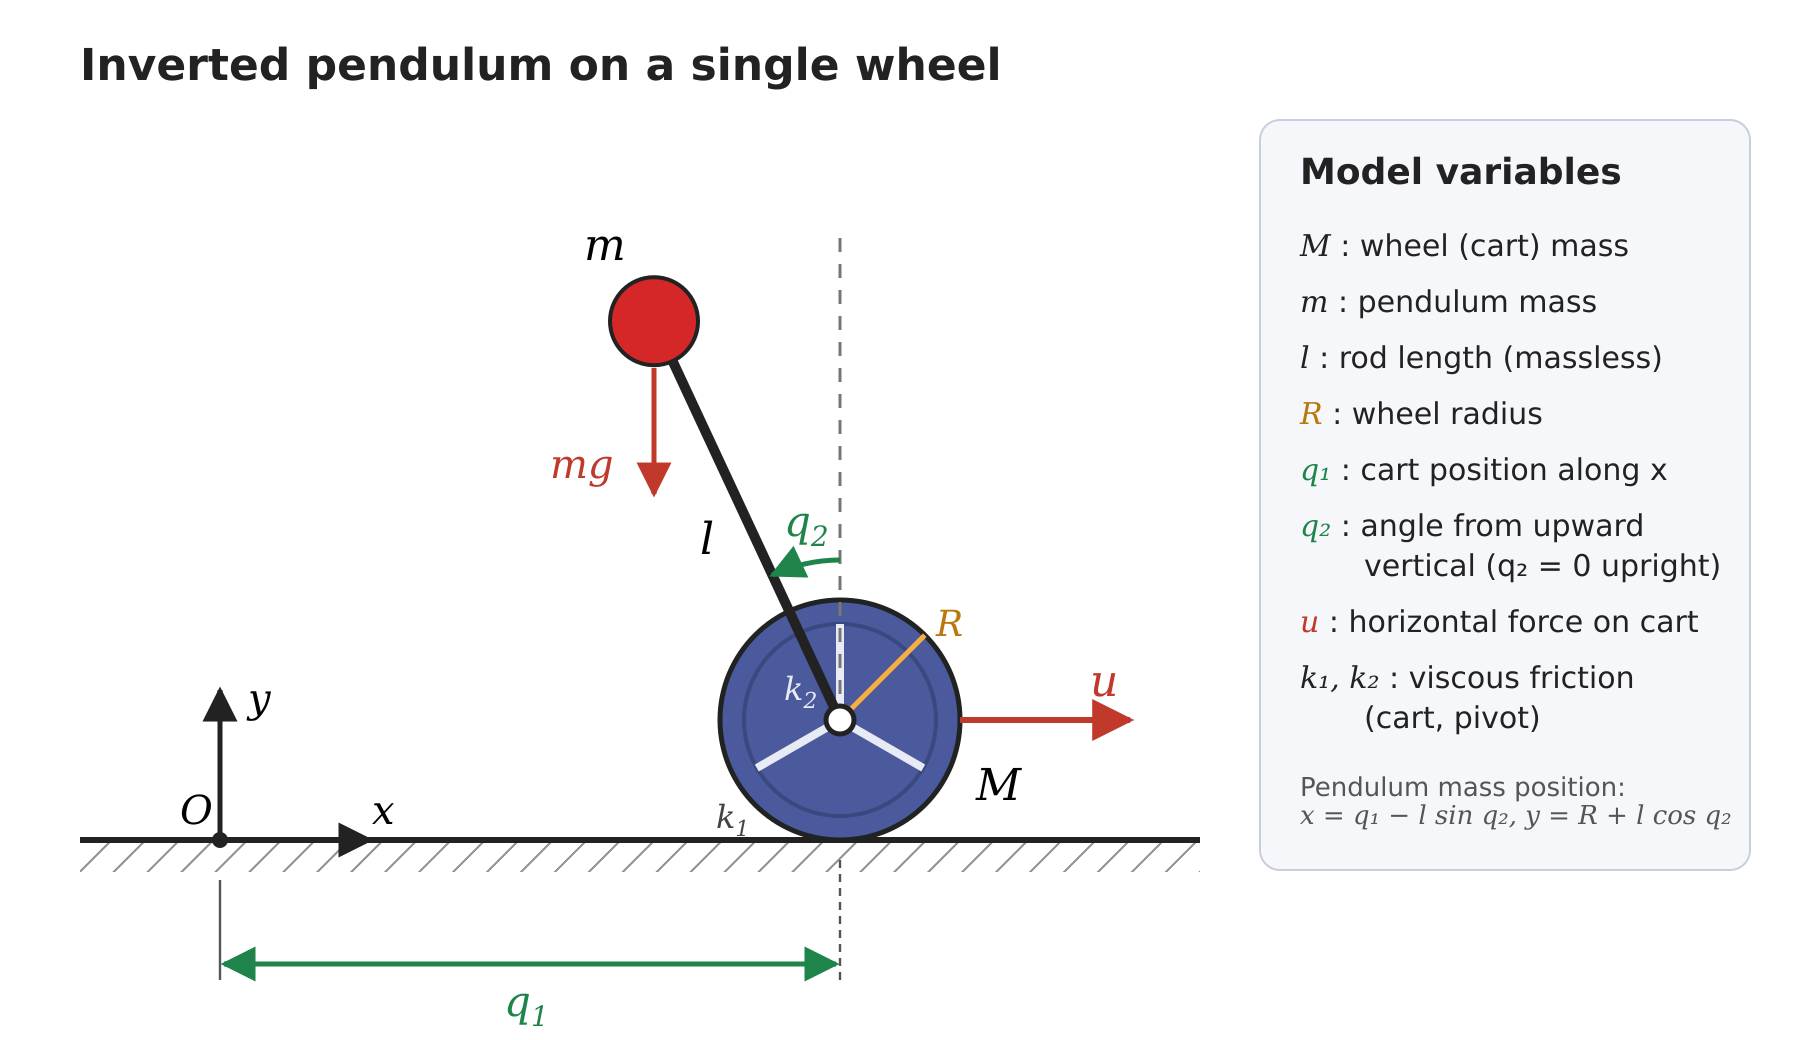
\includegraphics[width=\maxwidth{72.15253386853989em}]{image_0}
\end{center}
\end{par}

\begin{par}
\begin{flushleft}
The goal of the system is to stabilize the pendulum upright, keeping the swing angle q2 = 0 by controlling the displacement q1 of the car. 
\end{flushleft}
\end{par}


\vspace{1em}
\matlabtableofcontents{Table of Contents}

\vspace{1em}
\label{TMP_6f79}
\matlabheadingtwo{1. Model of the system}

\begin{par}
\begin{flushleft}
The system has 2 degrees of freedom q1 and q2. 
\end{flushleft}
\end{par}

\begin{par}
\begin{flushleft}
Considering the (x,y) frame the position of the masses are given as 
\end{flushleft}
\end{par}

\begin{par}
$$\left\lbrace \begin{array}{ll}
\vec{\mathrm{OM}\;}  & =q_1 \vec{\;x} \\
\vec{\;\mathrm{Om}}  & =\left(q_1 -l\;\sin \left(q_2 \right)\right)\;\vec{x} +l\;\cos \left(q_2 \right)\;\vec{\;y} 
\end{array}\right.$$
\end{par}


\vspace{1em}
\begin{par}
\begin{flushleft}
The velocities are:
\end{flushleft}
\end{par}

\begin{par}
$$\left\lbrace \begin{array}{ll}
\frac{d\vec{\;\mathrm{OM}} }{\mathrm{dt}} & =\dot{\;q_1 } \;\vec{\;x} \\
\frac{d\;\vec{\;\mathrm{Om}} }{\mathrm{dt}} & =\left(\dot{\;q_1 } +l\dot{\;q_2 } \;\cos \left(q_2 \right)\right)\vec{\;x} -l{\dot{\;q} }_2 \sin \left(q_2 \right)\;\vec{\;y} 
\end{array}\right.$$
\end{par}


\vspace{1em}
\begin{par}
\begin{flushleft}
The kinetic energy of the system is given as 
\end{flushleft}
\end{par}

\begin{par}
$$\begin{array}{l}
T=\frac{1}{2}M\times v_M^2 +\frac{\;1}{2}m\times v_{m\;}^2 =\frac{\;1}{2}M{\dot{\;q_1 } }^2 +\frac{1}{2}{m\left(\left(\dot{\;q_1 } +l\dot{\;q_2 } \;\cos \left(q_2 \right)\right)\vec{\;x} -l{\dot{\;q} }_2 \sin \left(q_2 \right)\;\vec{\;y} \right)}^2 \\
T=\frac{1}{2}\left(M+m\right){\dot{\;q_1 } }^2 +\frac{1}{2}m\left({l^2 \dot{\;q_2 } }^2 -2l\dot{\;q_1 } \dot{\;q_2 } \cos \left(q_2 \right)\right)
\end{array}$$ 
\end{par}

\begin{par}
\begin{flushleft}
The potential energy of the system is produced only by the mass m as the mass M is already grounded. So we have
\end{flushleft}
\end{par}

\begin{par}
$$V=\mathrm{m}\mathrm{g}\mathrm{L}\mathrm{c}\mathrm{o}\mathrm{s}\left(q_2 \right)\;$$
\end{par}


\vspace{1em}
\begin{par}
\begin{flushleft}
From the above energy equations, we obtain the Lagrangian
\end{flushleft}
\end{par}

\begin{par}
$$L=T-V=\frac{1}{2}\left(M+m\right){\dot{\;q_1 } }^2 +\frac{1}{2}m\left({l^2 \dot{\;q_2 } }^2 -2l\dot{\;q_1 } \dot{\;q_2 } \cos \left(q_2 \right)\right)-\mathrm{mgLcos}\left(q_2 \right)\;\;$$
\end{par}

\begin{par}
\begin{flushleft}
As the system is not only conservative. It also has dissipation force (friction of the contact between wheel and ground), generalized Lagrange equations apply as follows: 
\end{flushleft}
\end{par}

\begin{par}
$$\frac{d}{\mathrm{dt}}\left(\frac{\partial \;L}{\partial \;\dot{\;q_i } }\right)-\frac{\partial \;L}{\partial \;q_i }=Q_i$$
\end{par}

\begin{par}
\begin{flushleft}
Rayleigh dissipation function will be used to introduce the friction force proportional to velocity. 
\end{flushleft}
\end{par}

\begin{par}
$$R\left(\dot{\;q} \right)=\frac{1}{2}\sum_i^N k_i {\;\dot{\;q_i } }^2 =\frac{1}{2}\;\left(k_1 {\dot{\;q_1 } }^2 +k_2 \;{\dot{\;q_2 } }^2 \right)$$
\end{par}

\begin{par}
\begin{flushleft}
the dissipation force is given as $F_i =-\frac{\partial R}{\partial \dot{\;q_i } }\;\;\;;F_1 =-\frac{\partial R}{\partial \dot{\;q_1 } }=-\frac{1}{2}*\left({2*k}_1 \;\dot{\;q_1 } \right)=-k_1 \;\dot{q_1 }$
\end{flushleft}
\end{par}

\begin{par}
\begin{flushleft}
Thus $Q_i \;=F_i +<\mathrm{other}\;\mathrm{external}\;\mathrm{forces}\;\mathrm{applied}\;\mathrm{to}\;\mathrm{particle}\;i>$
\end{flushleft}
\end{par}

\begin{itemize}
\setlength{\itemsep}{-1ex}
   \item{\begin{flushleft} Lagrange equation w.r.t. $q_1$  \end{flushleft}}
\end{itemize}


\vspace{1em}
\begin{par}
$$\frac{d}{\mathrm{dt}}\left(\frac{\partial \;L}{\partial \;\dot{\;q_1 } }\right)-\frac{\partial \;L}{\partial \;q_1 }=-k_1 \;\dot{\;q_1 } +u$$ 
\end{par}

\begin{par}
\begin{flushleft}
$\frac{\partial \;L}{\partial \;\dot{\;q_1 } }=\left(M+m\right)\dot{\;q_1 } -m\;l\;\dot{q_2 } \;\cos \left(q_2 \right)\;$;   
\end{flushleft}
\end{par}

\begin{par}
$$\frac{d}{\mathrm{dt}}\left(\frac{\partial \;L}{\partial \;\dot{\;q_1 } }\right)=\left(M+m\right)\ddot{\;q_1 } -m\;l\ddot{\;q_2 } \;\cos \left(q_2 \right)+m\;l\;{\dot{q_2 } }^2 \;\sin \left(q_2 \right)$$
\end{par}

\begin{par}
$$\frac{\partial \;L}{\partial \;q_1 }=0$$
\end{par}

\begin{par}
$$\Rightarrow \frac{d}{\mathrm{dt}}\left(\frac{\partial \;L}{\partial \;\dot{\;q_1 } }\right)-\frac{\partial \;L}{\partial \;q_1 }=-k\;\dot{\;q_1 } \;\;\Rightarrow \left(M+m\right)\ddot{\;q_1 } -m\;l\ddot{\;q_2 } \;\cos \left(q_2 \right)+m\;l\;{\dot{q_2 } }^2 \;\sin \left(q_2 \right)+k_1 \;\dot{\;q_1 } =u$$
\end{par}


\vspace{1em}
\begin{itemize}
\setlength{\itemsep}{-1ex}
   \item{\begin{flushleft} Lagrange equation w.r.t. $q_2$ \end{flushleft}}
\end{itemize}

\begin{par}
$$\;\Rightarrow -m\;l\;\ddot{\;q_1 } \;\cos \left(q_2 \right)+m\;l^{2\;} \ddot{\;q_2 } -m\;g\;l\;\sin \left(q_2 \right)=-k_2 \;\dot{\;q_2 } \;$$
\end{par}


\vspace{1em}

\vspace{1em}
\begin{par}
\begin{flushleft}
The model of the system is given as 
\end{flushleft}
\end{par}

\begin{par}
$$\left\lbrace \begin{array}{ll}
\;\left(M+m\right)\ddot{\;q_1 } -m\;l\ddot{\;q_2 } \;\cos \left(q_2 \right)+m\;l\;{\dot{q_2 } }^2 \;\sin \left(q_2 \right)+k_1 \;\dot{\;q_1 }  & =u\\
-m\;l\;\ddot{\;q_1 } \;\cos \left(q_2 \right)+m\;l^{2\;} \ddot{\;q_2 } -m\;g\;l\;\sin \left(q_2 \right)+k_2 \;\dot{\;q_2 } \; & =0
\end{array}\right.$$
\end{par}


\vspace{1em}
\label{TMP_2298}
\matlabheadingtwo{2. Model linearization}

\begin{par}
\begin{flushleft}
 
\end{flushleft}
\end{par}

\begin{par}
$$\begin{array}{l}
q_2 \approx 0\approx \epsilon \;\\
\dot{\;q_2 \;} \approx \epsilon \;\;
\end{array}$$ $$\Rightarrow {\dot{q_2 } }^2 =\epsilon^2 \;\;;{\dot{q_2 } }^2 q_2 =\epsilon^3 =0$$
\end{par}

\begin{par}
$$q_2 \approx 0\;\Rightarrow \left\lbrace \begin{array}{ll}
\cos \left(q_2 \right) & \approx 1\\
\sin \left(q_2 \right) & \approx q_2 
\end{array}\right.$$ 
\end{par}


\vspace{1em}
\begin{par}
$$\Rightarrow \left\lbrace \begin{array}{ll}
\;\left(M+m\right)\ddot{\;q_1 } -m\;l\ddot{\;q_2 } \;+k_1 \;\dot{\;q_1 }  & =u\\
-m\;l\;\ddot{\;q_1 } \;+m\;l^{2\;} \ddot{\;q_2 } -m\;g\;l\;q_2 +k_2 \;\dot{\;q_2 } \; & =0
\end{array}\right.$$ 
\end{par}


\vspace{1em}
\begin{par}
$$\Rightarrow \left\lbrace \begin{array}{cc}
\ddot{\;q_1 }  & =\frac{\;m\;l\;}{M+m}\ddot{\;q_2 } -\frac{k_1 }{M+m}\;\dot{\;q_1 } \;+\frac{1}{M+m}u\;\;\;\;\;\;\;\;\;\;\;\\
\ddot{\;q_2 }  & \;=\frac{\;1}{l}\ddot{\;q_1 } -\frac{\;k_2 }{m\;l^2 }\dot{\;q_2 } +\frac{\;g}{l}q_2 \;\;\;\;\;\;\;\;\;\;\;\;\;\;\;\;\;\;\;\;\;\;\;\;\;\;\;\;\;\;\;\;\;\;\;\;\;\;\;
\end{array}\right.$$ 
\end{par}


\vspace{1em}
\begin{par}
$$\Rightarrow \left\lbrace \begin{array}{cc}
\ddot{\;q_1 } = & \frac{\;m\;}{M+m}\ddot{\;q_1 } \;-\frac{k_2 }{\left(M+m\right)l}\dot{\;q_2 } \;+\frac{\;m\;g}{\left(M+m\right)}q_2 \;-\frac{k_1 }{M+m}\dot{\;q_1 } +\frac{1}{M+m}u\\
\ddot{\;q_2 } = & \frac{\;m}{M+m}\ddot{\;q_2 } \;-\frac{\;k_1 }{\left(M+m\right)l}\dot{\;q_1 } -\frac{\;k_2 }{m\;l^2 }\dot{\;q_2 } +\frac{\;g}{l}q_2 +\frac{\;1}{\left(M+m\right)l\;}\;u\;\;\;\;\;\;\;\;\;\;\;\;\;\;\;\;\;\;\;\;\;\;\;\;\;\;\;\;\;\;\;\;\;\;\;
\end{array}\right.$$
\end{par}


\vspace{1em}
\begin{par}
$$\Rightarrow \left\lbrace \begin{array}{cc}
M\ddot{\;q_1 } = & -k_1 \dot{\;q_1 } -\frac{k_2 }{l}\dot{\;q_2 } \;+m\;g\;q_2 \;+u\;\;\;\;\;\;\;\;\;\;\;\;\;\;\;\;\;\;\;\;\;\;\;\;\;\;\;\;\;\;\;\;\;\;\;\;\;\;\;\;\;\;\;\;\;\;\;\\
M\ddot{\;q_2 } = & \;-\frac{\;k_1 }{l}\dot{\;q_1 } -\frac{\left(M+m\right)\;k_2 }{m\;l^2 }\dot{\;q_2 } +\frac{\;\left(M+m\right)g}{l}q_2 +\frac{1}{l}u\;
\end{array}\right.$$
\end{par}


\vspace{1em}
\begin{par}
$$\Rightarrow \left\lbrace \begin{array}{cc}
\ddot{\;q_1 } = & -\frac{k_1 }{M}\dot{\;q_1 } -\frac{k_2 }{M\;l\;}\dot{\;q_2 } \;+\frac{\;m\;g}{M\;}q_2 \;+\frac{\;1}{M}u\;\;\;\;\;\;\;\;\;\;\;\;\;\;\;\;\;\;\;\;\;\;\;\;\;\;\;\;\;\;\;\;\;\;\;\;\;\;\;\;\;\;\\
\ddot{\;q_2 } = & \;-\frac{\;k_1 }{M\;l}\dot{\;q_1 } -\frac{\left(M+m\right)\;k_2 }{M\;m\;l^2 }\dot{\;q_2 } +\frac{\;\left(M+m\right)g}{M\;l}q_2 +\frac{1}{M\;l}u\;\;
\end{array}\right.$$
\end{par}

\begin{par}
$$\;$$
\end{par}

\begin{par}
$$\Rightarrow \left\lbrace \begin{array}{ll}
\dot{\;q_1 }  & =\dot{\;q_1 } \\
\dot{\;q_2 }  & =\dot{\;q_2 } \\
\ddot{\;q_1 }  & =-\frac{k_1 }{M}\dot{\;q_1 } -\frac{k_2 }{M\;l}\dot{\;q_2 } \;+\frac{\;m\;g}{M\;l}q_2 \;+\frac{\;1}{M\;}u\\
\ddot{\;q_2 }  & =\;-\frac{\;k_1 }{M\;l}\dot{\;q_1 } -\frac{\left(M+m\right)\;k_2 }{M\;m\;l^2 }\dot{\;q_2 } +\frac{\;\left(M+m\right)g}{M\;l}q_2 +\frac{1}{M\;l}u\;\;\;\;\;
\end{array}\;\right.$$ 
\end{par}


\vspace{1em}
\begin{par}
$$\left\lbrack \begin{array}{c}
\dot{\;q_1 } \\
\dot{\;q_2 } \\
\ddot{\;q_1 } \\
\ddot{\;q_2 } 
\end{array}\right\rbrack =\left\lbrack \begin{array}{cccc}
0 & 0 & 1 & 0\\
0 & 0 & 0 & 1\\
0 & \frac{\;m\;g}{M\;} & -\frac{\;k_1 }{M} & -\frac{\;k_2 }{M\;l}\\
0 & \frac{\;\left(M+m\right)g}{M\;l} & -\frac{\;k_1 }{M\;l} & -\frac{\left(M+m\right)\;k_2 }{M\;m\;l^2 }
\end{array}\right\rbrack \left\lbrack \begin{array}{c}
q_1 \\
q_2 \\
\dot{\;q_1 } \\
\dot{\;q_2 } 
\end{array}\right\rbrack +\left\lbrack \begin{array}{c}
0\\
0\\
\frac{\;1}{M\;}\\
\frac{1}{M\;l}
\end{array}\right\rbrack u$$
\end{par}


\vspace{1em}

\vspace{1em}
\label{TMP_384f}
\matlabheadingtwo{3. Simulink Model of the system}

\begin{par}
\begin{flushleft}
The following values will taken for the system parameters
\end{flushleft}
\end{par}

\begin{par}
\begin{flushleft}
$M=1\ldotp 5\;\mathrm{kg}\;,m=0\ldotp 5\;\mathrm{kg},\;g=9\ldotp 81\;m/s\;,\;l=1\;m,{\;k}_1 =k_2 =0\ldotp 01$, 
\end{flushleft}
\end{par}

\begin{par}
\begin{flushleft}
We will take $q_2 =y$ as the output of the system
\end{flushleft}
\end{par}


\begin{matlabcode}
clear all
close all
clc
\end{matlabcode}


\begin{matlabcode}


run("parameters.m");

[plant_ss, plant_tf, plant_zpk] = syst_repr_generator(params, 'q2');
plant_ss.StateName = {'q_1', 'q_2', '\dot{q_1}', '\dot{q_2}'}; 
q20 = 10;
Tsim = 10;
% plant_ss
plant_tf
\end{matlabcode}
\begin{matlaboutput}
plant_tf = 
     0.6667 s^2 + 1.4e-17 s + 6.598e-16
  ----------------------------------------
  s^4 + 0.03333 s^3 - 13.08 s^2 - 0.0654 s
 
Continuous-time transfer function.
Model Properties
\end{matlaboutput}
\begin{matlabcode}
dcgain(plant_tf)
\end{matlabcode}
\begin{matlaboutput}
ans = Inf
\end{matlaboutput}
\begin{matlabcode}

plant_zpk
\end{matlabcode}
\begin{matlaboutput}
plant_zpk = 
            0.66667 s
  -----------------------------
  (s+3.631) (s-3.602) (s+0.005)
 
Continuous-time zero/pole/gain model.
Model Properties
\end{matlaboutput}
\begin{matlabcode}

\end{matlabcode}

\begin{par}
\begin{flushleft}
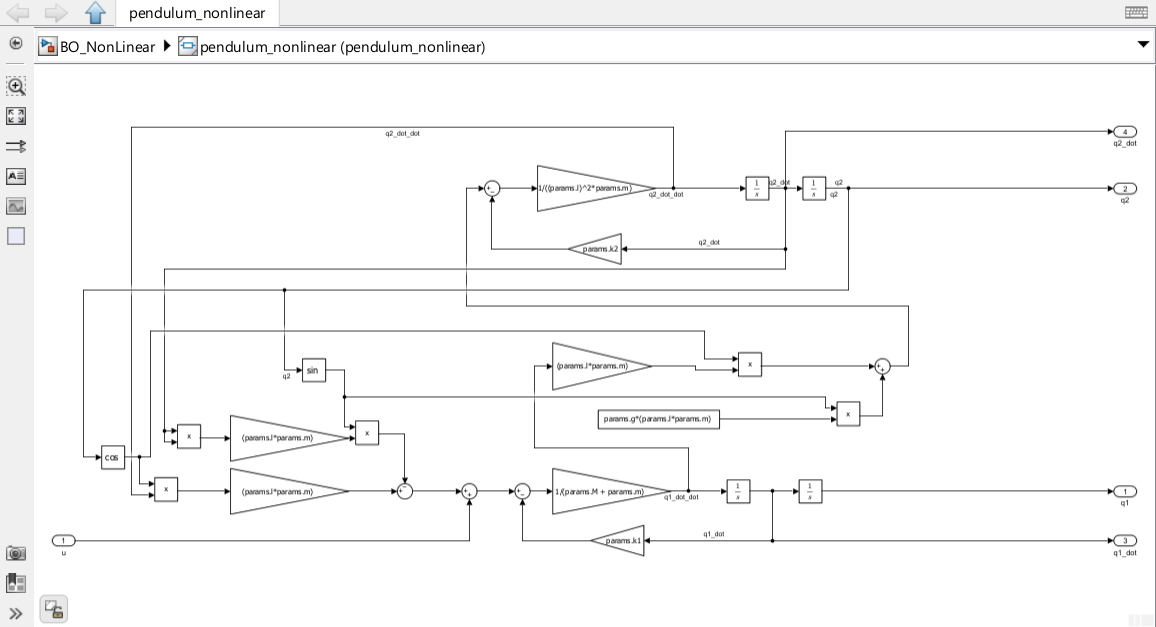
\includegraphics[width=\maxwidth{74.05920722528852em}]{image_1}
\end{flushleft}
\end{par}

\begin{par}
\begin{flushleft}
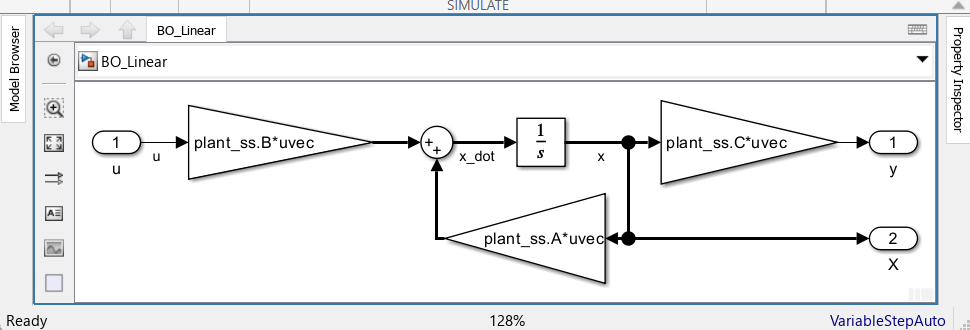
\includegraphics[width=\maxwidth{51.48018063221274em}]{image_2}
\end{flushleft}
\end{par}


\label{TMP_5f4a}
\matlabheadingtwo{4. System analysis}

\label{TMP_1ab7}
\vspace{1em}

\begin{par}
\begin{flushleft}
 
\end{flushleft}
\end{par}

\label{TMP_13e9}
\matlabheadingthree{Stability}

\begin{par}
\hfill \break
\end{par}

\begin{matlabcode}
[plant_ss, plant_tf, plant_zpk] = syst_repr_generator(params, 'q2');

poles_syst = pole(plant_ss)
\end{matlabcode}
\begin{matlaboutput}
poles_syst = 4x1

-3.6308    
3.6025     
-0.0050    
0          

\end{matlaboutput}
\begin{matlabcode}
zeros_syst = zero(plant_ss)
\end{matlabcode}
\begin{matlaboutput}
zeros_syst = 2x1
1.0e+-16
0.4043    
0         

\end{matlaboutput}
\begin{matlabcode}
clf("reset")
figure
pzmap(plant_ss)
\end{matlabcode}
\begin{center}
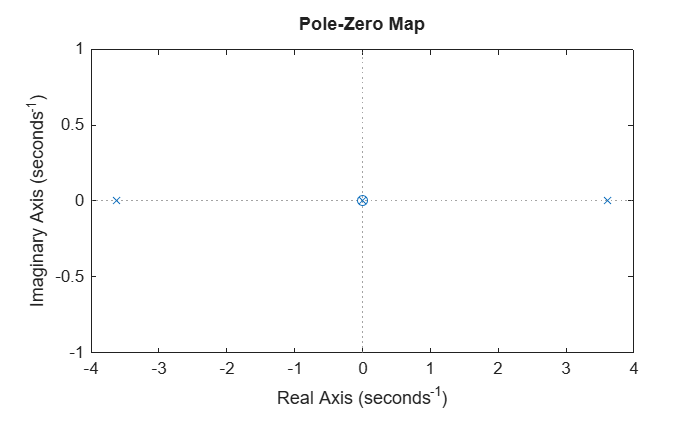
\includegraphics[width=\maxwidth{56.196688409433015em}]{figure_0.png}
\end{center}
\begin{matlabcode}
[plant_ss, plant_tf, plant_zpk] = syst_repr_generator(params, 'q1');
zeros_syst = zero(plant_ss)
\end{matlabcode}
\begin{matlaboutput}
zeros_syst = 2x1

3.1221     
-3.1421    

\end{matlaboutput}

\begin{par}
\begin{flushleft}
The system is unstable because the second pole of the system is a real positive.
\end{flushleft}
\end{par}

\begin{par}
\begin{flushleft}
The transfer function from u to q2 has a zero at the origin (s = 0). It cancels the open-loop pole at the origin, which is why the reduced transfer function has 3 poles and 1 zero. From u to the cart position q1 there is a right-half-plane zero at s=3.1221, so the system is non-minimum phase with respect to q1.
\end{flushleft}
\end{par}

\label{TMP_2110}
\vspace{1em}

\begin{matlabcode}
[plant_ss, plant_tf, plant_zpk] = syst_repr_generator(params, 'q2');

clf("reset")
figure 
rlocus(plant_ss)
\end{matlabcode}
\begin{center}
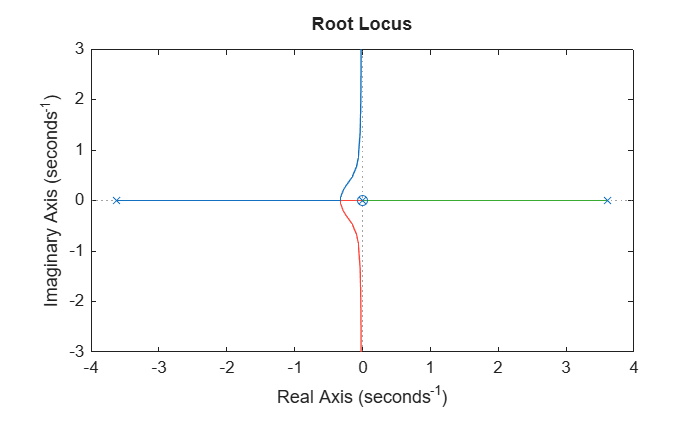
\includegraphics[width=\maxwidth{56.196688409433015em}]{figure_1.png}
\end{center}

\begin{par}
$$O\;L\;\left(s\right)=\frac{N}{D}\;\;\;;P\;\mathrm{ctrl}\;;\Rightarrow C\;L\;\left(s\right)=\frac{P\;N}{D+P\;N\;\;}$$
\end{par}

\begin{par}
\begin{flushleft}
A proportional controller alone cannot stabilize the system. The transfer function has 3 poles and 1 zero, located at the origin. As the gain increases, the unstable pole (s = +3.60) moves along the real axis towards that zero, so it never enters the left half-plane. Therefore no finite P gain can stabilize the system.
\end{flushleft}
\end{par}


\vspace{1em}
\label{TMP_44e2}
\vspace{1em}

\label{TMP_4085}
\matlabheadingthree{Controllability and observability}

\begin{par}
\hfill \break
\end{par}

\begin{matlabcode}
run parameters.m
[plant_ss_q1] = syst_repr_generator(params,'q1');
[plant_ss_q2] = syst_repr_generator(params,'q2');
plant_ss = plant_ss_q1;
Qc = ctrb(plant_ss);

rc = rank(Qc)
\end{matlabcode}
\begin{matlaboutput}
rc = 4
\end{matlaboutput}
\begin{matlabcode}
ro_q1 = rank(obsv(plant_ss_q1))
\end{matlabcode}
\begin{matlaboutput}
ro_q1 = 4
\end{matlaboutput}
\begin{matlabcode}
ro_q2 = rank(obsv(plant_ss_q2))
\end{matlabcode}
\begin{matlaboutput}
ro_q2 = 3
\end{matlaboutput}
\begin{matlabcode}

\end{matlabcode}

\begin{par}
\begin{flushleft}
The system is controllable as the rank of the controllability matrix is equal to the dimension of the A. 
\end{flushleft}
\end{par}

\begin{par}
\begin{flushleft}
$r_o =3\not= \dim \left(A\right)=4$, the system is not observable when $q_2$ is chosen as the output of the system. However it becomes observable for $q_1$as output 
\end{flushleft}
\end{par}


\vspace{1em}
\begin{matlabcode}
plant_ss_diag = diagonalize(plant_ss)
\end{matlabcode}
\begin{matlaboutput}
plant_ss_diag = 
  A = 
           x1      x2      x3      x4
   x1       0       0       0       0
   x2       0  -3.631       0       0
   x3       0       0   3.602       0
   x4       0       0       0  -0.005
 
  B = 
           u1
   x1     100
   x2  0.3583
   x3  0.3547
   x4    -100
 
  C = 
             x1        x2        x3        x4
   y1         1  -0.06448   0.06479         1
 
  D = 
       u1
   y1   0
 
Continuous-time state-space model.
Model Properties
\end{matlaboutput}

\begin{par}
\begin{flushleft}
By diagonalizing the LTI model, we can directly see that all the states are controllable as B matrix is full. 
\end{flushleft}
\end{par}


\vspace{1em}

\label{TMP_0911}
\matlabheadingtwo{5.Control }

\label{TMP_565c}
\matlabheadingthree{Loop shaping with PID controller }

\begin{enumerate}
\setlength{\itemsep}{-1ex}
   \item{\begin{flushleft} \textbf{u to q2  (q2 as output)} \end{flushleft}}
\end{enumerate}

\begin{par}
\begin{flushleft}
In this section simulink Control System Designer tool is used to tune a PID controller that stabilize the pendulum. 
\end{flushleft}
\end{par}

\begin{par}
\begin{flushleft}
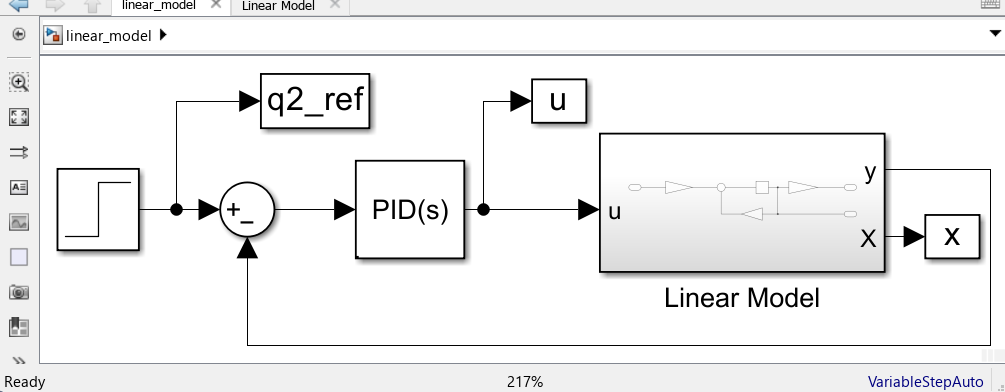
\includegraphics[width=\maxwidth{33.416959357752134em}]{image_3}
\end{flushleft}
\end{par}

\begin{par}
\begin{flushleft}
For the simulation $q_{20} =10\degree$
\end{flushleft}
\end{par}

\begin{matlabcode}
Tsim = 10;
Ts = 1e-4;
q2_f = deg2rad(-10);
params.IC = [0,deg2rad(1),0,0];
model = 2; % 1 : linear model,   2: non linear model  , 3: Matlab fct non linear model
[plant_ss] = syst_repr_generator(params,'q2');
input_select = plant_ss.C(1:2);
sim("models/mdl_with_PID.slx");
\end{matlabcode}
\begin{matlaboutput}
Warning: Model 'mdl_with_PID' contains 1 algebraic loops. 
Suggested Actions:
    • Highlight and view information about the algebraic loops in the model using the Simulink.BlockDiagram.getAlgebraicLoops function. - Open
    • Suppress this diagnostic by setting the 'Algebraic Loop' diagnostic parameter to 'none'. - Fix

\end{matlaboutput}
\begin{matlabcode}
refs = {'q1_ref', 'q2_ref'};

X = states_from_log(x);              
animate_pendulum_cart(x.Time, X(:,1), X(:,2), u.Data, params, 'fps', 100, ...
    string(refs(input_select==1)), ref.Data*input_select', 'model', model);
\end{matlabcode}
\begin{center}
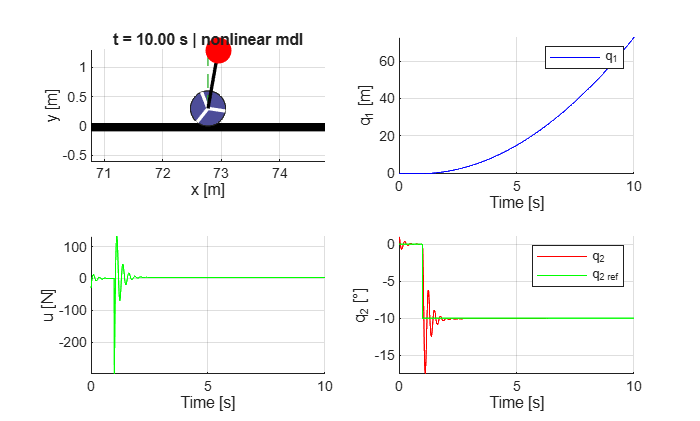
\includegraphics[width=\maxwidth{56.196688409433015em}]{figure_2.png}
\end{center}

\begin{par}
\begin{flushleft}
By using simulink blocks to model the non-linear system, we encounter algebraic loops because ${\ddot{q} }_1$requires  ${\ddot{q} }_2$ and vice-versa. To solve that, we will use Matlab function block (src/pendulum\_cart\_nl.m), to solve the following ode. 
\end{flushleft}
\end{par}

\begin{par}
$$\left\lbrace \begin{array}{ll}
\;\left(M+m\right)\ddot{\;q_1 } -m\;l\ddot{\;q_2 } \;\cos \left(q_2 \right)+m\;l\;{\dot{q_2 } }^2 \;\sin \left(q_2 \right)+k_1 \;\dot{\;q_1 }  & =u\\
-m\;l\;\ddot{\;q_1 } \;\cos \left(q_2 \right)+m\;l^{2\;} \ddot{\;q_2 } -m\;g\;l\;\sin \left(q_2 \right)+k_2 \;\dot{\;q_2 } \; & =0
\end{array}\;\;\;\;\;=\Rightarrow \left\lbrace \begin{array}{ll}
\;\left(M+m\right)\ddot{\;q_1 } -m\;l\ddot{\;q_2 } \;\cos \left(q_2 \right) & =u-m\;l\;{\dot{q_2 } }^2 \;\sin \left(q_2 \right)-k_1 \;\dot{\;q_1 } \\
-m\;l\;\ddot{\;q_1 } \;\cos \left(q_2 \right)+m\;l^{2\;} \ddot{\;q_2 } \; & =m\;g\;l\;\sin \left(q_2 \right)-k_2 \;\dot{\;q_2 } 
\end{array}\;\;\;\;\;\;\right.\right.$$ 
\end{par}

\begin{par}
$$\left\lbrack \begin{array}{c}
\ddot{\;q_1 } \\
\ddot{\;q_2 } 
\end{array}\right\rbrack ={\left\lbrack \begin{array}{cccc}
\left(M+m\right) & -m\;l\;\cos \left(q_2 \right)\\
-m\;l\;\cos \left(q_2 \right) & m\;l^{2\;} 
\end{array}\right\rbrack }^{-1} \;\left\lbrack \begin{array}{c}
\dot{\;u-m\;l\;{\dot{q_2 } }^2 \;\sin \left(q_2 \right)-k_1 \;\dot{\;q_1 } } \\
\dot{\;m\;g\;l\;\sin \left(q_2 \right)-k_2 \;\dot{\;q_2 } } 
\end{array}\right\rbrack$$
\end{par}


\label{TMP_130c}
\matlabheadingthree{Model validation}

\begin{itemize}
\setlength{\itemsep}{-1ex}
   \item{\begin{flushleft} \textbf{Open-loop fall test}  \end{flushleft}}
\end{itemize}

\begin{matlabcode}
run parameters.m
x0 = [0; deg2rad(0.5); 0; 0];
[t, x] = ode45(@(t,x) pendulum_cart_nl(x, 0, params), [0 50], x0);
clf("reset")
figure
plot(t, rad2deg(x(:,2))); grid on; xlabel('t [s]'); ylabel('q_2 [deg]')
\end{matlabcode}
\begin{center}
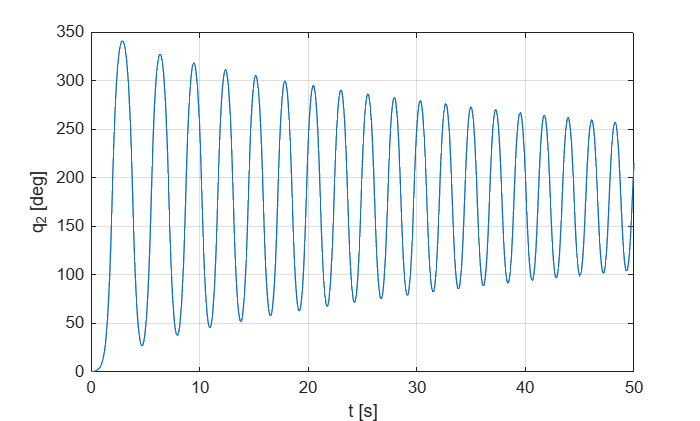
\includegraphics[width=\maxwidth{56.196688409433015em}]{figure_3.png}
\end{center}

\begin{par}
\begin{flushleft}
We can see that $q_2$is near 0 at about 1s, and then starts swinging with more and more low amplitude around 180°. 
\end{flushleft}
\end{par}


\vspace{1em}
\begin{itemize}
\setlength{\itemsep}{-1ex}
   \item{\begin{flushleft} \textbf{linear vs nonlinear at small angle} \end{flushleft}}
\end{itemize}

\begin{matlabcode}

plant = syst_repr_generator(params, 'q2');
t  = linspace(0, 0.8, 801)';
[~, ~, xl] = initial(plant, x0, t);
[~, xn]    = ode45(@(t,x) pendulum_cart_nl(x, 0, params), t, x0);
clf("reset")
figure
plot(t, rad2deg(xl(:,2)), t, rad2deg(xn(:,2)), '--'); 
legend('linear', 'nonlinear'); xlabel('t [s]'); ylabel('q_2 [deg]')
\end{matlabcode}
\begin{center}
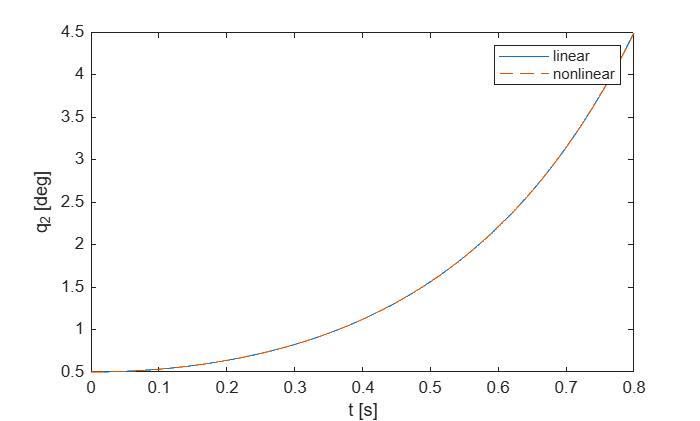
\includegraphics[width=\maxwidth{56.196688409433015em}]{figure_4.png}
\end{center}
\begin{matlabcode}
relErr = abs(xn(end,2) - xl(end,2)) / abs(xl(end,2))
\end{matlabcode}
\begin{matlaboutput}
relErr = 6.6129e-04
\end{matlaboutput}

\begin{par}
\begin{flushleft}
Linear and non-linear q2 output perfectly overlay with a relative error nearly null. 
\end{flushleft}
\end{par}


\vspace{1em}
\begin{itemize}
\setlength{\itemsep}{-1ex}
   \item{\begin{flushleft} \textbf{Linear model (variant 1) vs block model (variant 2) vs MATLAB Function (variant 3)} \end{flushleft}}
\end{itemize}

\begin{matlabcode}
run parameters.m
plant_ss = syst_repr_generator(params, 'q2');
input_select = plant_ss.C(1:2);
Tsim = 10;  Ts = 1e-4;  q2_f = deg2rad(-10);
params.IC = [0, deg2rad(1), 0, 0];
clf("reset")
figure; hold on; grid on
for model = 1:3                       % 1 linear, 2 blocks, 3 MATLAB Function
    out = sim("mdl_with_PID");
    X = states_from_log(x);
    Xs{model} = X;
    plot(x.Time, rad2deg(X(:,2)), 'DisplayName', "model " + model)

end
\end{matlabcode}
\begin{matlaboutput}
Warning: Model 'mdl_with_PID' contains 1 algebraic loops. 
Suggested Actions:
    • Highlight and view information about the algebraic loops in the model using the Simulink.BlockDiagram.getAlgebraicLoops function. - Open
    • Suppress this diagnostic by setting the 'Algebraic Loop' diagnostic parameter to 'none'. - Fix

\end{matlaboutput}
\begin{matlabcode}
maxDiff_2vs3 = max(abs(rad2deg(Xs{2}(:,2) - Xs{3}(:,2))))   
\end{matlabcode}
\begin{matlaboutput}
maxDiff_2vs3 = 0.0192
\end{matlaboutput}
\begin{matlabcode}
maxDiff_1vs3 = max(abs(rad2deg(Xs{1}(:,2) - Xs{3}(:,2))))   
\end{matlabcode}
\begin{matlaboutput}
maxDiff_1vs3 = 0.6567
\end{matlaboutput}
\begin{matlabcode}
legend; xlabel('t [s]'); ylabel('q_2 [deg]')
\end{matlabcode}
\begin{center}
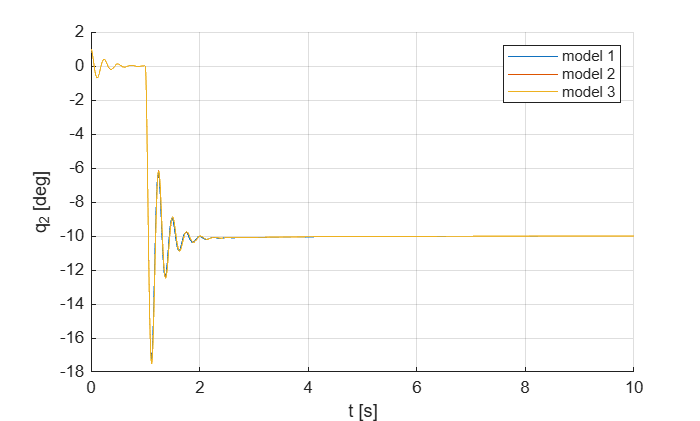
\includegraphics[width=\maxwidth{56.196688409433015em}]{figure_5.png}
\end{center}

\begin{par}
\begin{flushleft}
The nonlinear model was implemented twice: as a Simulink block diagram and as a MATLAB Function solving the mass-matrix form of the Lagrange equations. Under the same PID scenario (q₂₀ = 1°, step to −10°), the two implementations differ by at most 0.019° over 10 s, which confirms both. The linear model differs from them by at most 0.66°, about 4\% of the 17° peak, consistent with the small-angle approximation at that amplitude.
\end{flushleft}
\end{par}


\begin{par}
\begin{flushleft}
Getting back to PID control this time with MATLAB function based nonlinear model. 
\end{flushleft}
\end{par}

\begin{matlabcode}

Tsim = 10;
Ts = 1e-4;
q2_f = deg2rad(-10);
params.IC = [0,deg2rad(1),0,0];
model = 3; % 1 : linear model,   2: non linear model  , 3: Matlab fct non linear model
[plant_ss] = syst_repr_generator(params,'q2');
input_select = plant_ss.C(1:2);
sim("models/mdl_with_PID.slx");
refs = {'q1_ref', 'q2_ref'};

X = states_from_log(x);              
animate_pendulum_cart(x.Time, X(:,1), X(:,2), u.Data, params, 'fps', 100, ...
    string(refs(input_select==1)), ref.Data*input_select', 'model', model);
\end{matlabcode}
\begin{center}
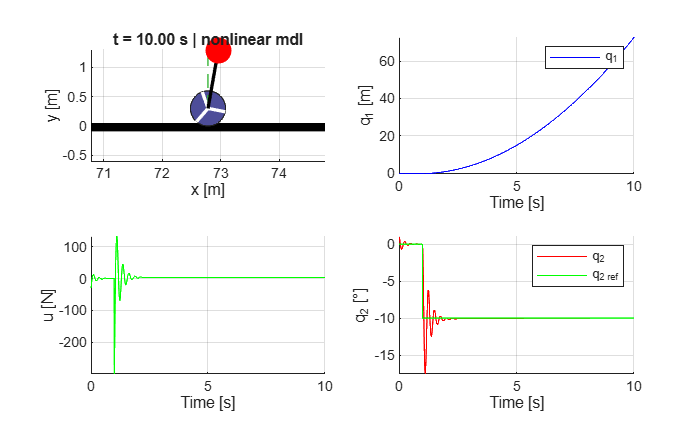
\includegraphics[width=\maxwidth{56.196688409433015em}]{figure_6.png}
\end{center}
\begin{matlabcode}

\end{matlabcode}

\begin{par}
\begin{flushleft}
The PID controller assured the pendulum cart to move as desired. Actually holding $q_2$  constant (${\dot{q} }_2 =0$ and ${\ddot{\;q} }_2 =0$) at -10° needs a constant acceleration of the cart, ${\ddot{\;q} }_1 =a=-g\ldotp \tan \left(q_2 \right)\approx 1\ldotp 73\;m/s^2$. So the cart position $q_1$ grows like a parabola  ($\approx 70\;m\;\mathrm{in}\;9\;s$) and u settles at  $\left(M+m\right)\cdot a\approx 3\ldotp 5N$
\end{flushleft}
\end{par}


\begin{matlabcode}

\end{matlabcode}

\begin{itemize}
\setlength{\itemsep}{-1ex}
   \item{\begin{flushleft} \textbf{u to q1 (q1 as output)} \end{flushleft}}
\end{itemize}

\begin{matlabcode}
Tsim = 10;
Ts = 1e-4;
q2_f = deg2rad(-10);
params.IC = [0,deg2rad(1),0,0];
model = 1; % 1 : linear model,   2: non linear model  , 3: Matlab fct non linear model
[plant_ss] = syst_repr_generator(params,'q1');
input_select = plant_ss.C(1:2);
sim("models/mdl_with_PID.slx");
refs = {'q1_ref', 'q2_ref'};

X = states_from_log(x);              
animate_pendulum_cart(x.Time, X(:,1), X(:,2), u.Data, params, 'fps', 100, ...
    string(refs(input_select==1)), ref.Data*input_select', 'model', model);
\end{matlabcode}
\begin{center}
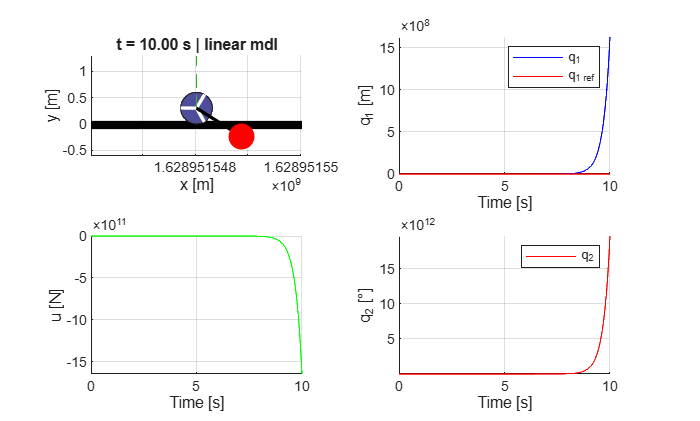
\includegraphics[width=\maxwidth{56.196688409433015em}]{figure_7.png}
\end{center}


\label{TMP_7b2d}
\matlabheadingthree{State feedback control}

\begin{par}
\begin{flushleft}
This control law is expressed as $u=-Kx+k_{\mathrm{s}\mathrm{c}\mathrm{a}\mathrm{l}\mathrm{e}} \;y_{\mathrm{r}\mathrm{e}\mathrm{f}}$
\end{flushleft}
\end{par}

\begin{par}
\begin{flushleft}
Classical state feedback controller is only applicable to SISO system, so we have to choose one of the two possible outputs
\end{flushleft}
\end{par}

\label{TMP_4886}
\matlabheadingthree{State feedback controller with cart position (q\_1) as output }

\begin{par}
\begin{flushleft}
By default we will set $k_{\mathrm{s}\mathrm{c}\mathrm{a}\mathrm{l}\mathrm{e}} =1$
\end{flushleft}
\end{par}

\begin{matlabcode}
[plant_ss]  = syst_repr_generator(params,'q1');
poles_des = [-3, -3, -3, -3];
rank(plant_ss.B);
K = acker(plant_ss.A,plant_ss.B, poles_des);
Tsim = 20;
Ts = 1e-4;
q2_f = deg2rad(10);
params.IC = [0,deg2rad(20),0,0];
model = 3; % 1 : linear model       2: non linear model    3: Matlab fct non linear model
k_scale = 1;
input_select = plant_ss.C(1:2);
refs = {'q1_ref', 'q2_ref'};
sim('models/mdl_with_State_Feedback.slx');
X = states_from_log(x);              
animate_pendulum_cart(x.Time, X(:,1), X(:,2), u.Data, params, 'fps', 100, ...
    string(refs(input_select==1)), ref.Data*input_select', 'model', model);
\end{matlabcode}
\begin{center}
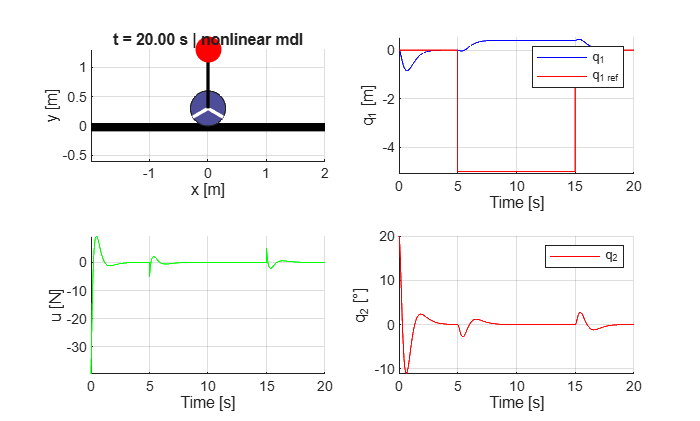
\includegraphics[width=\maxwidth{56.196688409433015em}]{figure_8.png}
\end{center}
\begin{matlabcode}

\end{matlabcode}

\begin{par}
\begin{flushleft}
With the compensator $k_{\mathrm{scale}}$ set to default 1, a state feedback controller cannot assure a null static error.
\end{flushleft}
\end{par}


\begin{par}
\begin{flushleft}
To illustrate the compensator effect, let's consider a simple first order system with a static gain of 0.5. The step plot show a response ceiling at 0.5 instead of 1, the reference. With the compensator, the output is scaled to catch the reference. The same principle is used in state feedback controller.
\end{flushleft}
\end{par}

\begin{matlabcode}
s = zpk('s');
toy_system = 2/(4 + s)
\end{matlabcode}
\begin{matlaboutput}
toy_system = 
    2
  -----
  (s+4)
 
Continuous-time zero/pole/gain model.
Model Properties
\end{matlaboutput}
\begin{matlabcode}
clf(gcf)
figure
step(toy_system)
\end{matlabcode}
\begin{center}
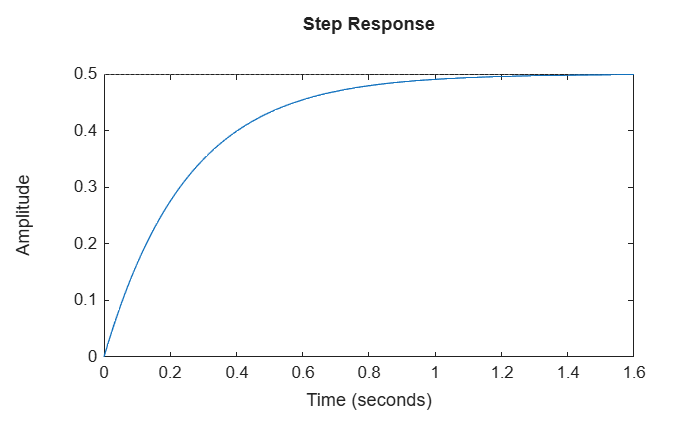
\includegraphics[width=\maxwidth{56.196688409433015em}]{figure_9.png}
\end{center}
\begin{matlabcode}
figure
clf(gcf)
dcg = dcgain(toy_system)
\end{matlabcode}
\begin{matlaboutput}
dcg = 0.5000
\end{matlaboutput}
\begin{matlabcode}
compensator = 1/dcg
\end{matlabcode}
\begin{matlaboutput}
compensator = 2
\end{matlaboutput}
\begin{matlabcode}
step(compensator*toy_system)
\end{matlabcode}
\begin{center}
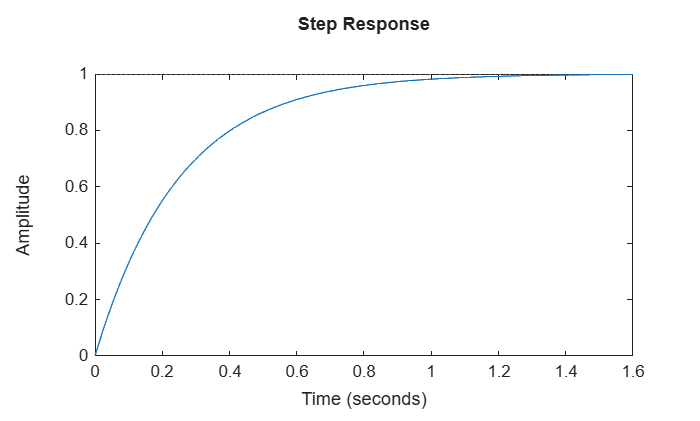
\includegraphics[width=\maxwidth{56.196688409433015em}]{figure_10.png}
\end{center}
\begin{matlabcode}

\end{matlabcode}


\begin{par}
\begin{flushleft}
By default we will set $k_{\mathrm{s}\mathrm{c}\mathrm{a}\mathrm{l}\mathrm{e}} =\frac{1}{\mathrm{d}\mathrm{c}\mathrm{g}\mathrm{a}\mathrm{i}\mathrm{n}\left(\mathrm{c}\mathrm{l}\mathrm{o}\mathrm{s}\mathrm{e}\mathrm{d}\;\mathrm{l}\mathrm{o}\mathrm{o}\mathrm{p}\right)}$
\end{flushleft}
\end{par}

\begin{matlabcode}
[plant_ss]  = syst_repr_generator(params,'q1');
poles_des = [-3, -3, -3, -3];
rank(plant_ss.B);
K = acker(plant_ss.A,plant_ss.B, poles_des);
Tsim = 20;
Ts = 1e-4;
q2_f = deg2rad(20);
params.IC = [0,deg2rad(20),0,0];
model = 3; % 1 : linear model       2: non linear model    3: Matlab fct non linear model

A_cl = plant_ss.A - plant_ss.B*K;
B_cl = plant_ss.B;
closed_loop_ss =  ss(A_cl, B_cl, plant_ss.C, 0);
[b,a] = ss2tf(A_cl,B_cl, plant_ss.C,0);
closed_loop_tf = tf(b,a)
\end{matlabcode}
\begin{matlaboutput}
closed_loop_tf = 
    0.6667 s^2 + 0.01333 s - 6.54
  ----------------------------------
  s^4 + 12 s^3 + 54 s^2 + 108 s + 81
 
Continuous-time transfer function.
Model Properties
\end{matlaboutput}
\begin{matlabcode}
dcg = dcgain(closed_loop_ss);
k_scale = 1/dcg;
input_select = plant_ss.C(1:2);
refs = {'q1_ref', 'q2_ref'};

sim('models/mdl_with_State_Feedback.slx');
clf("reset")
figure;
X = states_from_log(x);              
animate_pendulum_cart(x.Time, X(:,1), X(:,2), u.Data, params, 'fps', 100, ...
    string(refs(input_select==1)), ref.Data*input_select', 'model', model);
\end{matlabcode}
\begin{center}
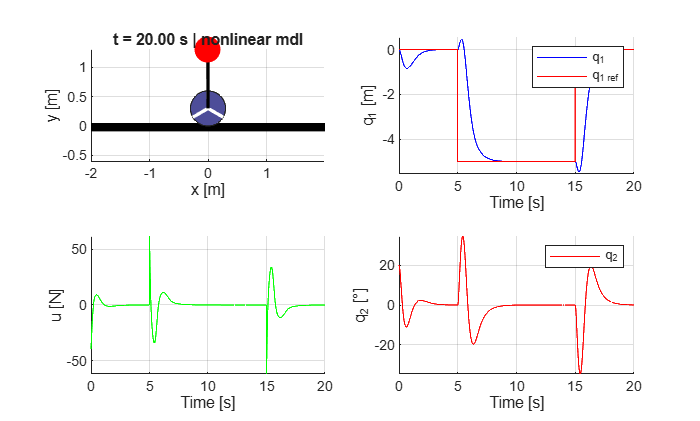
\includegraphics[width=\maxwidth{56.196688409433015em}]{figure_11.png}
\end{center}
\begin{matlabcode}

\end{matlabcode}


\begin{matlabcode}
Tsim = 10;
Ts = 1e-4;
q2_f = deg2rad(20);
params.IC = [0,deg2rad(20),0,0];
model = 3; % 1 : linear model       2: non linear model
input_select = plant_ss.C(1:2);
sim('models/mdl_with_State_Feedback.slx');
refs = {'q1_ref', 'q2_ref'};
clf("reset")
figure;
X = squeeze(x.Data);              
if size(X,1) == 4, X = X.'; end  
animate_pendulum_cart(x.Time, X(:,1), X(:,2), u.Data, params, 'fps', 100, ...
    string(refs(input_select==1)), ref.Data*input_select', 'model', model);
\end{matlabcode}
\begin{center}
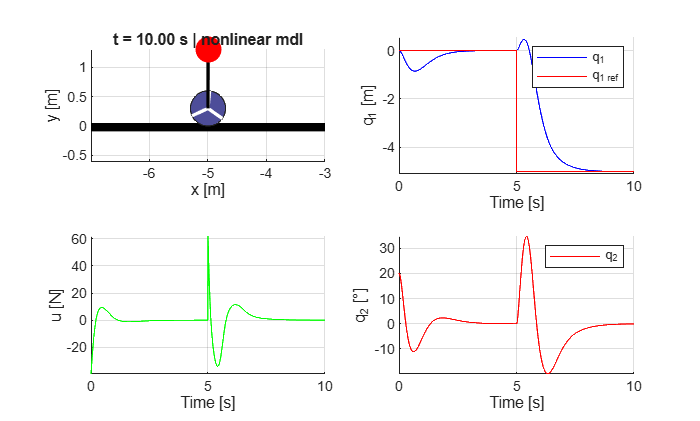
\includegraphics[width=\maxwidth{56.196688409433015em}]{figure_12.png}
\end{center}


\label{TMP_6a4a}
\matlabheadingthree{State feedback controller with swing angle (q\_2) as output }

\begin{par}
\begin{flushleft}
Taking $q_2$as output of the system reveals one of the implication of non observability show above. Actually, state feedback control only changes system's poles (the denominator of the the transfer function). Looking closely to the transfer function's numerator when $q_2$is the output, we notice that $b_0 =-1\ldotp 866e-16\approx 0$. This b0 ≈ 0 is the zero of u → q2 at s = 0: state feedback moves poles, never zeros, which result in $\mathrm{dcgain}=\frac{b_0 }{a_0 }\;$ being null and an infinite compensator $k_{\mathrm{scale}} =\infty$
\end{flushleft}
\end{par}

\begin{matlabcode}
[plant_ss]  = syst_repr_generator(params,'q2');
poles_des = [-3, -3, -3, -3];
rank(plant_ss.B);
K = acker(plant_ss.A,plant_ss.B, poles_des);
Tsim = 20;
Ts = 1e-4;
q2_f = deg2rad(20);
params.IC = [0,deg2rad(20),0,0];
model = 3; % 1 : linear model       2: non linear model    3: Matlab fct non linear model

A_cl = plant_ss.A - plant_ss.B*K;
B_cl = plant_ss.B;
closed_loop_ss =  ss(A_cl, B_cl, plant_ss.C, 0);
[b,a] = ss2tf(A_cl,B_cl, plant_ss.C,0);
closed_loop_tf = tf(b,a)
\end{matlabcode}
\begin{matlaboutput}
closed_loop_tf = 
  0.6667 s^2 + 1.668e-15 s - 1.866e-16
  ------------------------------------
   s^4 + 12 s^3 + 54 s^2 + 108 s + 81
 
Continuous-time transfer function.
Model Properties
\end{matlaboutput}
\begin{matlabcode}
dcg = dcgain(closed_loop_ss)
\end{matlabcode}
\begin{matlaboutput}
dcg = 0
\end{matlaboutput}
\begin{matlabcode}
k_scale = 1/dcg
\end{matlabcode}
\begin{matlaboutput}
k_scale = Inf
\end{matlaboutput}


\vspace{1em}

\label{TMP_2ff7}
\matlabheadingthree{LQR state feedback control}

\begin{par}
\hfill \break
\end{par}

\begin{matlabcode}
[plant_ss]  = syst_repr_generator(params,'q1');
Q = eye(4);       
R  =0.1;
K = lqr(plant_ss.A, plant_ss.B, Q, R);
A_cl = plant_ss.A - plant_ss.B*K;
B_cl = plant_ss.B;
closed_loop =  ss(A_cl, B_cl, plant_ss.C, 0);

dcg = dcgain(closed_loop);
k_scale = 1/dcg;
Tsim = 20;
Ts = 1e-4;
q2_f = deg2rad(10);
params.IC = [0,deg2rad(10),0,0];
model = 3; % 1 : linear model       2: non linear model    3: Matlab fct non linear model

input_select = plant_ss.C(1:2);
sim('models/mdl_with_State_Feedback.slx');
refs = {'q1_ref', 'q2_ref'};


X = states_from_log(x);              
animate_pendulum_cart(x.Time, X(:,1), X(:,2), u.Data, params, 'fps', 100, ...
    string(refs(input_select==1)), ref.Data*input_select', 'model', model);
\end{matlabcode}
\begin{center}
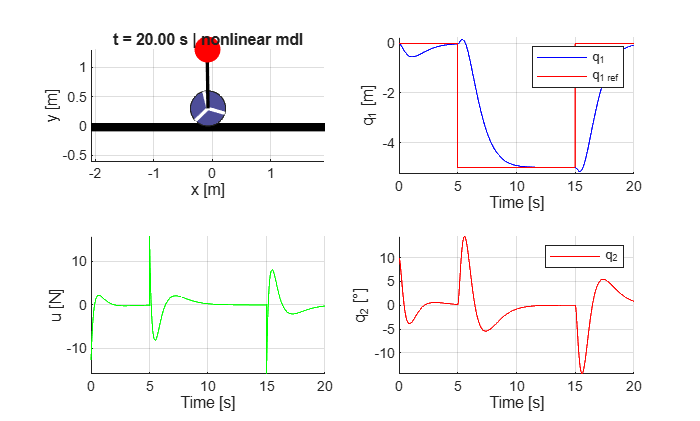
\includegraphics[width=\maxwidth{56.196688409433015em}]{figure_13.png}
\end{center}
\begin{matlabcode}

\end{matlabcode}


\label{TMP_6cfa}
\vspace{1em}

\label{TMP_8d2b}
\matlabheadingthree{Observer based state feedback control}

\begin{par}
\begin{flushleft}
In reality the state are not directly accessible. They are either measured using sensors or estimated with techniques such Luenberger for deterministic systems and Kalman filter for stochastic systems. 
\end{flushleft}
\end{par}

\begin{par}
\begin{flushleft}
In this exercise will first start with Luenberger observer.
\end{flushleft}
\end{par}

\begin{par}
\begin{flushleft}
This observer expressed the observed states as : 
\end{flushleft}
\end{par}

\begin{par}
\begin{flushleft}
$\dot{x_o } =A{\;x}_o +B\;u\;+L\left(y-y_o \right)$  ; $y_o =C\;x_o \;\;\mathrm{a}\mathrm{n}\mathrm{d}\;y=C\;x$ $\;\Rightarrow \;$$\dot{\;x_o } =\left(A-L\;C\right)\;x_o +B\;u+L\;y\;$ 
\end{flushleft}
\end{par}

\begin{par}
\begin{flushleft}
where $y_o \;\mathrm{and}\;y$ are respectively the observed and real output. L is the Luenberger gain that can be calculated via pole placement in order the guaranty a response time of the observer 5 to 10 times faster than the closed loop of the system. 
\end{flushleft}
\end{par}

\begin{matlabcode}

[plant_ss]  = syst_repr_generator(params,'q1');
poles_des = [-4, -3, -2.5, -1.2];
rank(plant_ss.B);
K = acker(plant_ss.A,plant_ss.B, poles_des);
Tsim = 20;
Ts = 1e-4;
q2_f = deg2rad(20);
params.IC = [0,deg2rad(20),0,0];
A_cl = plant_ss.A - plant_ss.B*K;
B_cl = plant_ss.B;
closed_loop =  ss(A_cl, B_cl, plant_ss.C, 0);
obsv_poles = [-15, -16, -17, -18];
L = place(plant_ss.A', plant_ss.C', obsv_poles)';
dcg = dcgain(closed_loop);
k_scale = 1/dcg;
input_select = plant_ss.C(1:2);
refs = {'q1_ref', 'q2_ref'};
model = 3;  % 1 : linear model       2: non linear model    3: Matlab fct non linear model
sim('models/mdl_with_State_Feedback_and_observer.slx');

X = states_from_log(x);              
animate_pendulum_cart(x.Time, X(:,1), X(:,2), u.Data, params, 'fps', 100, ...
    string(refs(input_select==1)), ref.Data*input_select', 'model', model);
\end{matlabcode}
\begin{center}
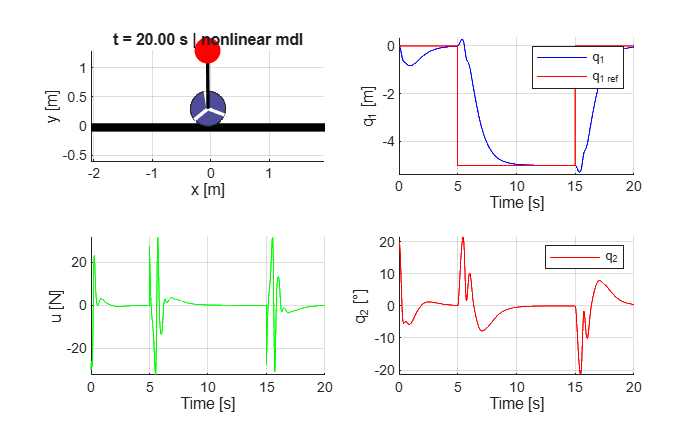
\includegraphics[width=\maxwidth{56.196688409433015em}]{figure_14.png}
\end{center}


\label{TMP_51d0}
\matlabheadingthree{States observer based-LQR State feedback with integral action }

\begin{itemize}
\setlength{\itemsep}{-1ex}
   \item{\begin{flushleft} \textbf{u to q2 (q2 as output)} \end{flushleft}}
\end{itemize}

\begin{par}
\begin{flushleft}
In order to assure that static error elimination on the pendulum angle, we are going to augment the controller with integral action. 
\end{flushleft}
\end{par}

\begin{matlabcode}
% Augmented system (integral action on q2)
[plant_ss]  = syst_repr_generator(params,'q2');
P = [plant_ss.A, zeros(4,1); -plant_ss.C, 0]; % -C_q2
Rin = [plant_ss.B; 0];
Q = 2*eye(5);
R = 2.5;
K_aug = lqr(P, Rin, Q, R);
P_cl = P - Rin*K_aug;
R_cl = Rin ;
rank(ctrb(P, Rin)) 
\end{matlabcode}
\begin{matlaboutput}
ans = 4
\end{matlaboutput}
\begin{matlabcode}
ss_cl =  ss(P_cl, R_cl, [plant_ss.C 0], 0);
pole(ss_cl)
\end{matlabcode}
\begin{matlaboutput}
ans = 5x1 complex

-3.9379 + 0.0000i    
-3.3400 + 0.0000i    
-0.5242 + 0.4122i    
-0.5242 - 0.4122i    
-0.0000 + 0.0000i    

\end{matlaboutput}
\begin{matlabcode}

Tsim = 20;
Ts = 1e-4;
params.IC = [0,deg2rad(1),0,0];
model = 3; % 1: linear model       2: non linear model    3: Matlab fct non linear model
input_select = [0,1]; 
q2_f = deg2rad(2);
refs = {"q1_ref", "q2_ref"};
sim('models/mdl_with_State_Feedback_integral.slx');

X = states_from_log(x);              
animate_pendulum_cart(x.Time, X(:,1), X(:,2), u.Data, params, 'fps', 100, ...
    string(refs(input_select==1)), ref.Data*input_select', 'model', model);
\end{matlabcode}
\begin{center}
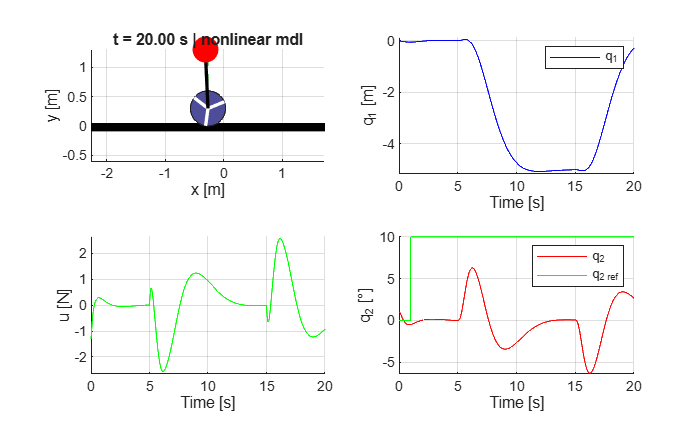
\includegraphics[width=\maxwidth{56.196688409433015em}]{figure_15.png}
\end{center}
\begin{matlabcode}

\end{matlabcode}

\begin{par}
\begin{flushleft}
The plant from u to q₂ has a zero at s = 0. In the augmented system, this zero cancels the pole of the integrator, so the augmented pair (P, Rin) is not controllable (rank 4 instead of 5). LQR can only place the four controllable poles; the uncontrollable mode remains at s = 0 (the −0.0000 pole). As a result, the controller stabilizes the pendulum but cannot make q₂ track the reference: q₂ returns to 0 while the cart drifts at constant speed and the integrator state grows without bound.
\end{flushleft}
\end{par}

\begin{par}
\begin{flushleft}
Physically, integral action requires a resting state where the output equals its reference, and a controllable augmented system. Neither holds here: holding q₂ ≠ 0 requires a constant cart acceleration, so no resting state exists, and the force acts on the wheel, never directly on the pendulum mass. Integral action is therefore applied to the cart position q₁ instead, where both conditions are met.
\end{flushleft}
\end{par}

\begin{matlabcode}

\end{matlabcode}


\begin{itemize}
\setlength{\itemsep}{-1ex}
   \item{\begin{flushleft} u to q1 (q1 as output) \end{flushleft}}
\end{itemize}

\begin{matlabcode}

plant_ss = syst_repr_generator(params, 'q1');
P   = [plant_ss.A, zeros(4,1); -plant_ss.C, 0];
Rin = [plant_ss.B; 0];
rank(ctrb(P, Rin))            % must be 5 (it is only 4 with q2)
\end{matlabcode}
\begin{matlaboutput}
ans = 5
\end{matlaboutput}
\begin{matlabcode}
Q = 10*eye(5);
R = 2.5;
K_aug = lqr(P, Rin, Q, R);
pole(ss(P - Rin*K_aug, Rin, [plant_ss.C 0], 0))   % all strictly negative
\end{matlabcode}
\begin{matlaboutput}
ans = 5x1 complex

-4.4139 + 0.0000i    
-3.0403 + 0.0000i    
-0.9866 + 0.0000i    
-0.7058 + 0.6999i    
-0.7058 - 0.6999i    

\end{matlaboutput}
\begin{matlabcode}
obsv_poles = [-15, -16, -17, -18];
L = place(plant_ss.A', plant_ss.C', obsv_poles)';
Tsim = 20;
Ts = 1e-4;
params.IC = [0,deg2rad(1),0,0];
model = 3; % 1: linear model       2: non linear model    3: Matlab fct non linear model
input_select = plant_ss.C(1:2);
q2_f = deg2rad(10);
refs = {"q1_ref", "q2_ref"};
sim('models/mdl_with_State_Feedback_integral_and_observer.slx')

X = states_from_log(x);              
animate_pendulum_cart(x.Time, X(:,1), X(:,2), u.Data, params, 'fps', 100, ...
    string(refs(input_select==1)), ref.Data*input_select', 'model', model);
\end{matlabcode}
\begin{center}
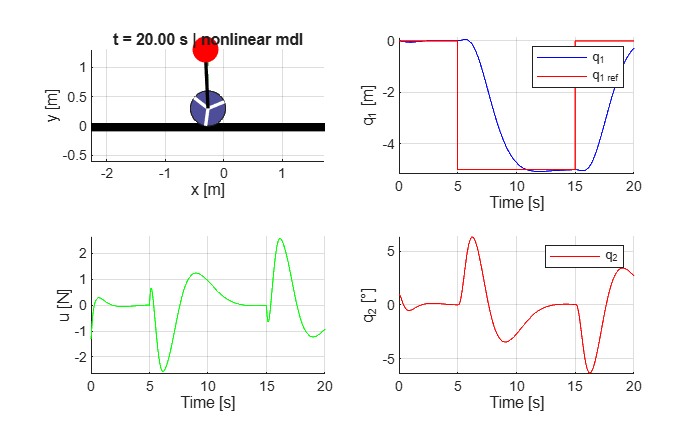
\includegraphics[width=\maxwidth{56.196688409433015em}]{figure_16.png}
\end{center}


\label{TMP_1df1}
\matlabheadingthree{Sliding mode control}

\begin{par}
\begin{flushleft}
Sliding mode control is a robust control strategy that aims to drag the system dynamic to a sliding surface $S\left(x\right)=F\;x-r$. The $r$ term is added to follow a reference $y_{\mathrm{ref}}$. 
\end{flushleft}
\end{par}

\begin{par}
\begin{flushleft}
The adapted reference r is determine as follows: 
\end{flushleft}
\end{par}

\begin{par}
\begin{flushleft}
On sliding surface $S\left(x_{\infty } \right)=0$
\end{flushleft}
\end{par}

\begin{par}
$$\left\lbrack \begin{array}{c}
{\dot{x} }_{\infty } \\
S\left(x_{\infty } \right)
\end{array}\right\rbrack =\left\lbrack \begin{array}{cc}
A & B\\
F & 0
\end{array}\right\rbrack \left\lbrack \begin{array}{c}
x_{\infty } \\
u_{\infty } 
\end{array}\right\rbrack +\left\lbrack \begin{array}{c}
0_{n\times 1} \\
-r
\end{array}\right\rbrack =\left\lbrack \begin{array}{c}
0_{n\times \;1} \\
0
\end{array}\right\rbrack$$
\end{par}

\begin{par}
\begin{flushleft}
let $M=\left\lbrack \begin{array}{cc}
A & B\\
F & 0
\end{array}\right\rbrack$ 
\end{flushleft}
\end{par}

\begin{par}
$$\left\lbrack \begin{array}{c}
x_{\infty } \\
u_{\infty } 
\end{array}\right\rbrack =r\;M^{-1} \left\lbrack \begin{array}{c}
0_{n\times \;1} \\
1
\end{array}\right\rbrack =r\;\left\lbrack \begin{array}{c}
x_t \\
u_t 
\end{array}\right\rbrack$$
\end{par}

\begin{par}
$$y_{\mathrm{ref}} =y_{\infty } =C\;x_{\infty } +D\;u_{\infty } =\left(C\;x_t +D\;u_t \right)\;r=\alpha \;r\Longrightarrow r=\frac{y_{\mathrm{ref}} }{\alpha }$$
\end{par}

\begin{par}
\begin{flushleft}
A generalized Ackerman pole placement method is used to calculate $F$, with a resulting Hurwitz caracteristic polynomial 
\end{flushleft}
\end{par}

\begin{par}
\begin{flushleft}
$\gamma \left(s\right)={\left(s+p\right)}^{n-k}$    with $n$, the order of the system and $k$, the relative degree that can be arbitrary choosing as long as the condition $k<n$ is met. $p\;$ is the only desired pole to choose. 
\end{flushleft}
\end{par}

\begin{par}
$$F=e_1 \;Q^{-1} \;\gamma \left(A\right)$$
\end{par}

\begin{par}
\begin{flushleft}
where $Q=\left\lbrack B\;\;\;A\;B\;\;\;\;\ldotp \ldotp \ldotp \;\;A^{n-1} B\right\rbrack$ the controllability matrix and $e_1 =\left\lbrack 0_{1\times \left(n-1\right)} \;\;\;1\right\rbrack$
\end{flushleft}
\end{par}


\vspace{1em}
\begin{par}
\begin{flushleft}
The control law $u\;$is given as 
\end{flushleft}
\end{par}

\begin{par}
$$u=-\frac{F\;A^k +f\left(\xi \;\right)}{F\;A^{k-1} \;B}$$ 
\end{par}

\begin{par}
\begin{flushleft}
$f\left(\xi \;\right)\;$is the discontinuous part of the controller chosen here as $f\left(\xi \;\right)=k_0 \;\tanh \left(\frac{S\left(x\right)}{\phi \;}\right)\;$. 
\end{flushleft}
\end{par}

\begin{par}
\begin{flushleft}
$\phi \;$defines the sliding coridor  
\end{flushleft}
\end{par}

\begin{par}
\begin{flushleft}
For more details refer to Debbie Hernández, Fernando Castaños, and Leonid Fridman. Pole-placement in higher-order sliding-mode control. In 19th IFAC World Congress, volume 47 of IFAC Proceedings Volumes, pages 1386–1391. IFAC
\end{flushleft}
\end{par}


\vspace{1em}
\begin{matlabcode}
run parameters.m
[plant_ss]  = syst_repr_generator(params,'q1');
Qc = ctrb(plant_ss.A,plant_ss.B);
e = [zeros(1,3) 1];
p = 3;
gamma = (plant_ss.A + p*eye(4))^3;
F = e*inv(Qc)*gamma; 
k0 = 20;
phi = 0.5;
q1_ref = 5; 
params.IC = [0,deg2rad(10),0,0];
q2_f = deg2rad(2);
M = [plant_ss.A, plant_ss.B; F, 0];
x_u_inf = M\[zeros(4,1); 1];
alpha = plant_ss.C*x_u_inf(1:end-1);
r = q1_ref/alpha; 
input_select = plant_ss.C(1:2);
Tsim = 20;
Ts=1e-4;
model = 3; % 1 : linear model       2: non linear model    3: Matlab fct non linear model
sim('models/mdl_with_SMC.slx');
refs = {'q1_ref', 'q2_ref'};

X = states_from_log(x);              
animate_pendulum_cart(x.Time, X(:,1), X(:,2), u.Data, params, 'fps', 100, ...
    string(refs(input_select==1)), ref.Data*input_select', 'model', model);
\end{matlabcode}
\begin{center}
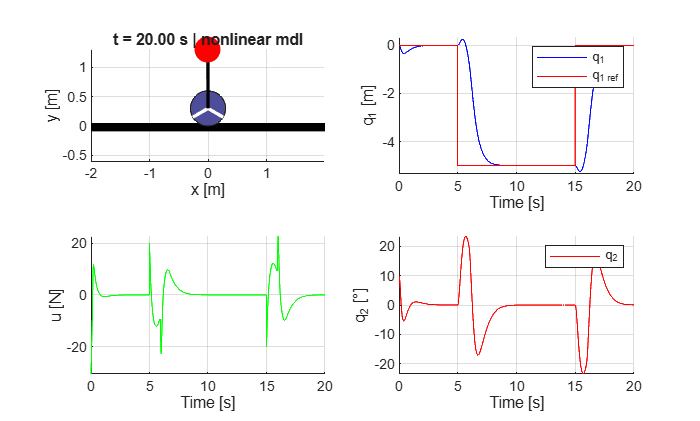
\includegraphics[width=\maxwidth{56.196688409433015em}]{figure_17.png}
\end{center}
\begin{matlabcode}
run parameters.m
[plant_ss]  = syst_repr_generator(params,'q1');
Qc = ctrb(plant_ss.A,plant_ss.B);
e = [zeros(1,3) 1];
p = 5;
gamma = (plant_ss.A + p*eye(4))^3;
F = e*inv(Qc)*gamma; 
k0 = 50;
phi = 0.5;
q1_ref = 5; 
params.IC = [0,deg2rad(10),0,0];
q2_f = deg2rad(2);
M = [plant_ss.A, plant_ss.B; F, 0];
x_u_inf = M\[zeros(4,1); 1];
alpha = plant_ss.C*x_u_inf(1:end-1);
r = q1_ref/alpha; 
input_select = plant_ss.C(1:2);
Tsim = 20;
Ts=1e-4;
model = 3; % 1 : linear model       2: non linear model    3: Matlab fct non linear model
sim('models/mdl_with_SMC.slx');
refs = {'q1_ref', 'q2_ref'};
X = states_from_log(x);              
animate_pendulum_cart(x.Time, X(:,1), X(:,2), u.Data, params, 'fps', 100, ...
    string(refs(input_select==1)), ref.Data*input_select', 'model', model);
\end{matlabcode}
\begin{center}
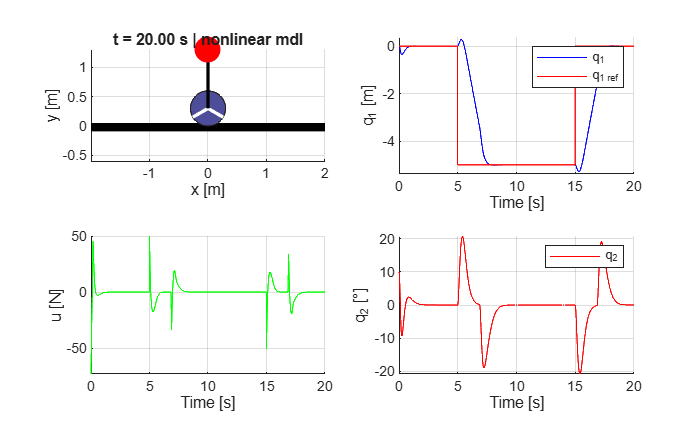
\includegraphics[width=\maxwidth{56.196688409433015em}]{figure_18.png}
\end{center}


\label{TMP_71ff}
\vspace{1em}

\end{document}
